\documentclass{article} % Класс печатного документа

\usepackage{graphicx}
\usepackage[utf8]{inputenc} % Кодировка исходного текста - utf8
\usepackage[english,russian]{babel} % Поддержка языка - русского с английским
\usepackage{indentfirst} % Отступ в первом абзаце

\title{Отчёт 6\protect\\Скрытые модели Маркова} % Заголовок документа
\author{Свичкарев А.\,В.} % Автор документа
\date{\today} % Текущая дата

\begin{document} % Конец преамбулы, начало текста

\maketitle % Печатает заголовок, список авторов и дату

\section{Задание №1}
Предсказание статусов (buried, exposed) для последовательности\newlineпротеина:

\begin{verbatim}
MYGKIIFVLLLSEIVSISASSTTGVAMHTSTSSSVTKSYISSQTNDTHKRDTYAATPRA
----*******--**------------------------*-------------------
HEVSEISVRTVYPPEEETGERVQLAHHFSEPEITLIIFGVMAGVIGTILLISYGIRRLI
-----***--*----------*----------***********************--**
KKSPSDVKPLPSPDTDVPLSSVEIENPETSDQ
------*-------------------------
\end{verbatim}

\section{Задание №2}
График вероятностей двух состояний аминокислот из заданной последовательности белка: buried (black) и exposed (grey) для каждой позиции марковской цепи:

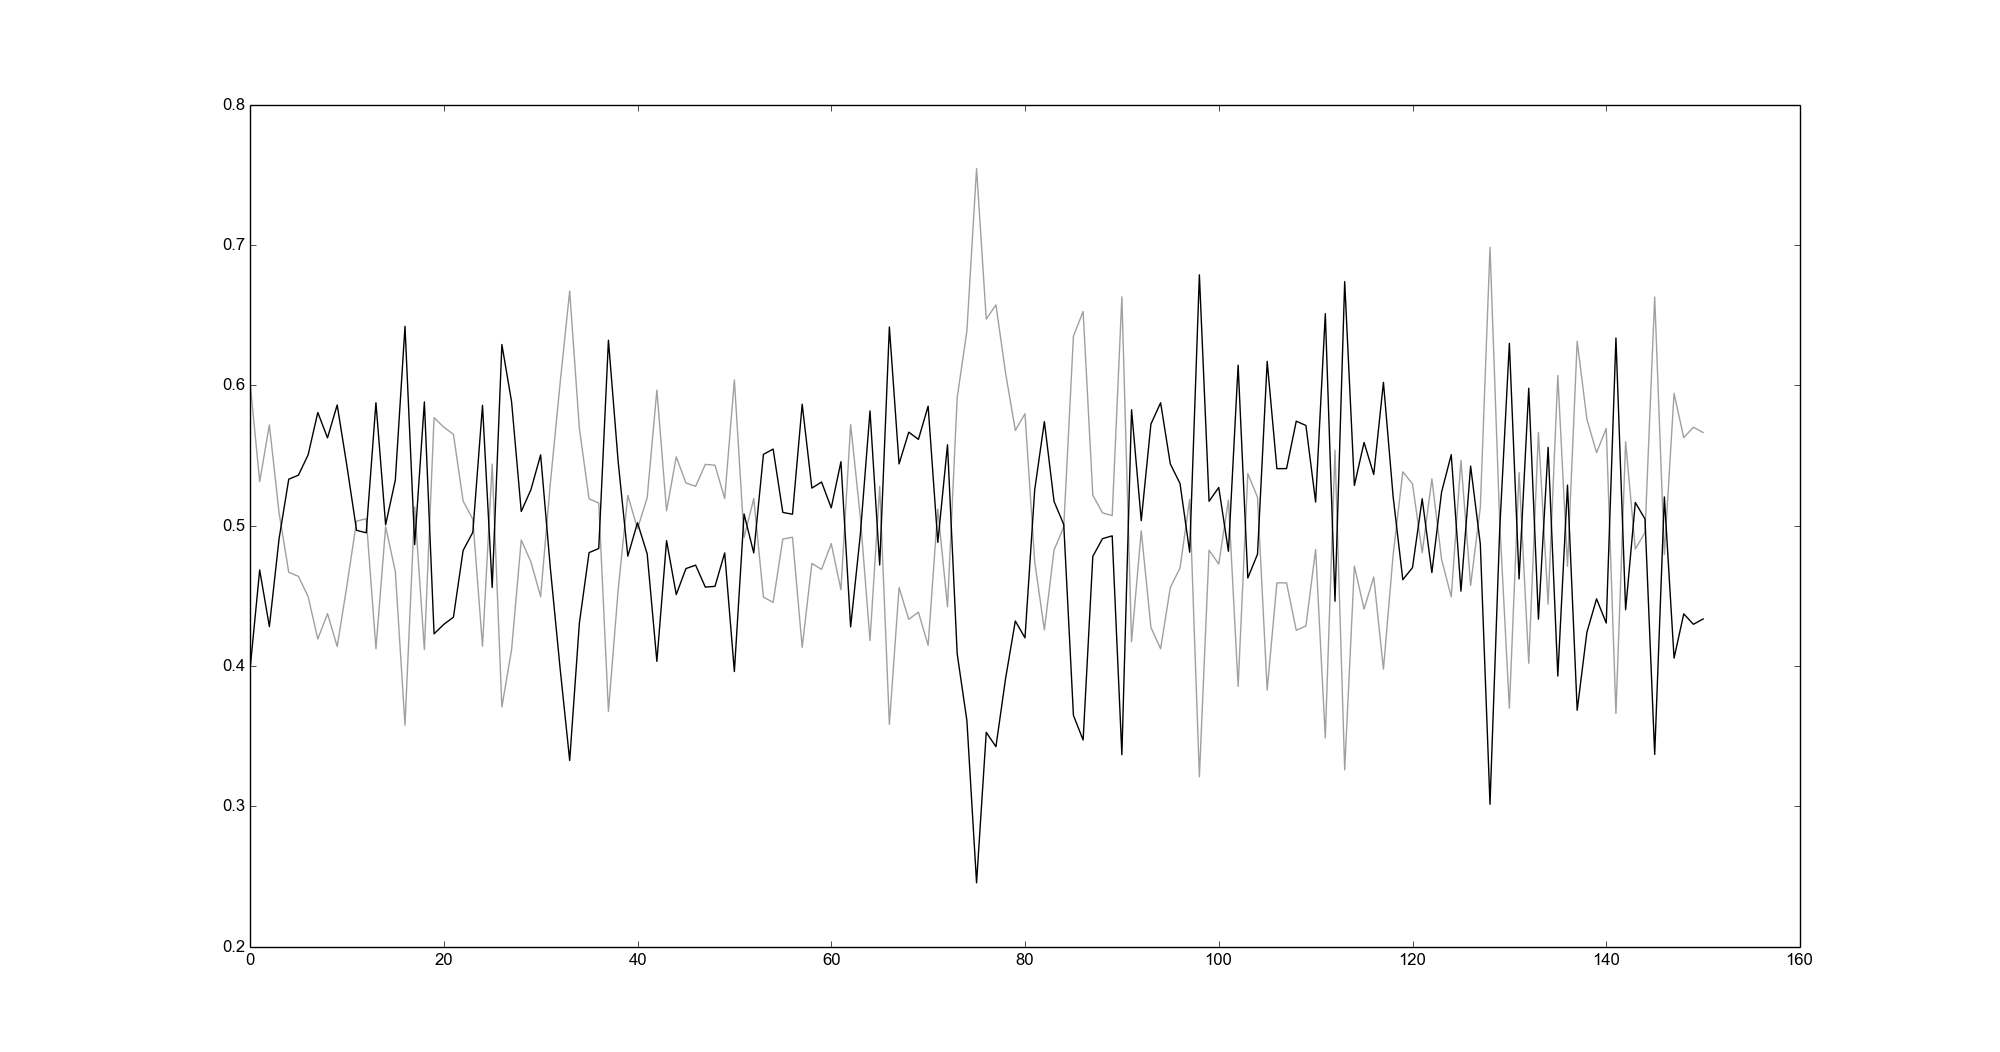
\includegraphics[width=\textwidth]{figure_1}

\end{document} % Конец документа
